%%%%%%%%%%%%%%%%%%%%%%%%%%%%%%%%%%%%%%%%%%%%%%%%%%%%%%%%%%%%%%%%%%
%%%%%%%%%%%%%%%%%%%%%%%%%%%%%%%%%%%%%%%%%%%%%%%%%%%%%%%%%%%%%%%%%%
% \setmathfont{TeX Gyre Termes Math}
%Packages
\documentclass[10pt, a4paper]{article}
\usepackage[top=3cm, bottom=4cm, left=2cm, right=2cm]{geometry}
\usepackage{amsmath,amsthm,amsfonts,amssymb,amscd, fancyhdr, color, comment, graphicx, environ}
\usepackage{float}
\usepackage{booktabs}
\usepackage{pifont}
\usepackage{mathrsfs}
\usepackage[math-style=ISO]{unicode-math}
\usepackage[dvipsnames]{xcolor}
\usepackage[framemethod=TikZ]{mdframed}
\usepackage{enumerate}
\usepackage[shortlabels]{enumitem}
\usepackage{fancyhdr}
\usepackage{indentfirst}
\usepackage{listings}
\usepackage{sectsty}
\usepackage{thmtools}
\usepackage{shadethm}
\usepackage{hyperref}
\usepackage{setspace}
\usepackage{adjustbox}
\hypersetup{
    colorlinks=true,
    linkcolor=blue,
    filecolor=magenta,      
    urlcolor=blue,
}
\usepackage{xcolor,colortbl}
%%%%%%%%%%%%%%%%%%%%%%%%%%%%%%%%%%%%%%%%%%%%%%%%%%%%%%%%%%%%%%%%%%
%%%%%%%%%%%%%%%%%%%%%%%%%%%%%%%%%%%%%%%%%%%%%%%%%%%%%%%%%%%%%%%%%%
%Environment setup
\mdfsetup{skipabove=\topskip,skipbelow=\topskip}
\newrobustcmd\ExampleText{%
An \textit{inhomogeneous linear} differential equation has the form
\begin{align}
L[v ] = f,
\end{align}
where $L$ is a linear differential operator, $v$ is the dependent
variable, and $f$ is a given nonzero function of the independent
variables alone.
}
\mdfdefinestyle{theoremstyle}{%
linecolor=black,linewidth=1pt,%
frametitlerule=true,%
frametitlebackgroundcolor=gray!20,
innertopmargin=\topskip,
}
\mdtheorem[style=theoremstyle]{Problem}{Question Number}
\setcounter{Problem}{5}
\newenvironment{Solution}{\textbf{Solution.}}

\definecolor{codegreen}{rgb}{0,0.6,0}
\definecolor{codegray}{rgb}{0.5,0.5,0.5}
\definecolor{codepurple}{rgb}{0.58,0,0.82}
\definecolor{backcolour}{rgb}{0.95,0.95,0.92}

\lstdefinestyle{mystyle}{
    backgroundcolor=\color{backcolour},   
    commentstyle=\color{codegreen},
    keywordstyle=\color{magenta},
    numberstyle=\tiny\color{codegray},
    stringstyle=\color{codepurple},
    basicstyle=\ttfamily\footnotesize,
    breakatwhitespace=false,         
    breaklines=true,                 
    captionpos=b,                    
    keepspaces=true,                 
    numbers=left,                    
    numbersep=5pt,                  
    showspaces=false,                
    showstringspaces=false,
    showtabs=false,                  
    tabsize=2
}

\lstset{style=mystyle}
%%%%%%%%%%%%%%%%%%%%%%%%%%%%%%%%%%%%%%%%%%%%%%%%%%%%%%%%%%%%%%%%%%
%%%%%%%%%%%%%%%%%%%%%%%%%%%%%%%%%%%%%%%%%%%%%%%%%%%%%%%%%%%%%%%%%%
%Fill in the appropriate information below
\newcommand{\norm}[1]{\left\lVert#1\right\rVert}     
\newcommand\course{XXXX0000}                            % <-- course name   
\newcommand\hwnumber{0}                                 % <-- homework number
\newcommand\Information{Someone}                        % <-- personal information
%%%%%%%%%%%%%%%%%%%%%%%%%%%%%%%%%%%%%%%%%%%%%%%%%%%%%%%%%%%%%%%%%%
%%%%%%%%%%%%%%%%%%%%%%%%%%%%%%%%%%%%%%%%%%%%%%%%%%%%%%%%%%%%%%%%%%
%Page setup
\pagestyle{fancy}
\headheight 35pt
\lhead{\today \hspace*{4cm} Key-Breakers}
\rhead{
\includegraphics[width=1.2cm]{../logo.png}}
\lfoot{}
\pagenumbering{arabic}
\cfoot{\small\thepage}
\rfoot{}
\headsep 1.2em
\renewcommand{\baselinestretch}{1.25}
%%%%%%%%%%%%%%%%%%%%%%%%%%%%%%%%%%%%%%%%%%%%%%%%%%%%%%%%%%%%%%%%%%
%%%%%%%%%%%%%%%%%%%%%%%%%%%%%%%%%%%%%%%%%%%%%%%%%%%%%%%%%%%%%%%%%%
%Add new commands here
\renewcommand{\labelenumi}{\alph{enumi})}
\newcommand{\Z}{\mathbb Z}
\newcommand{\R}{\mathbb R}
\newcommand{\Q}{\mathbb Q}
\newcommand{\NN}{\mathbb N}
\newcommand{\PP}{\mathbb P}
\DeclareMathOperator{\Mod}{Mod} 
\renewcommand\lstlistingname{Algorithm}
\renewcommand\lstlistlistingname{Algorithms}
\def\lstlistingautorefname{Alg.}
\newtheorem*{theorem}{Theorem}
\newtheorem*{lemma}{Lemma}
\newtheorem{case}{Case}
\newcommand{\assign}{:=}
\newcommand{\infixiff}{\text{ iff }}
\newcommand{\nobracket}{}
\newcommand{\backassign}{=:}
\newcommand{\tmmathbf}[1]{\ensuremath{\boldsymbol{#1}}}
\newcommand{\tmop}[1]{\ensuremath{\operatorname{#1}}}
\newcommand{\tmtextbf}[1]{\text{{\bfseries{#1}}}}
\newcommand{\tmtextit}[1]{\text{{\itshape{#1}}}}

\newenvironment{itemizedot}{
    \begin{itemize} 
    \renewcommand{\labelitemi}{$\bullet$}
    \renewcommand{\labelitemii}{$\bullet$}
    \renewcommand{\labelitemiii}{$\bullet$}
    \renewcommand{\labelitemiv}{$\bullet$}}
    {\end{itemize}}

\catcode`\<=\active\def<{
\fontencoding{T1}\selectfont\symbol{60}\fontencoding{\encodingdefault}}
\catcode`\>=\active\def>{
\fontencoding{T1}\selectfont\symbol{62}\fontencoding{\encodingdefault}}
\catcode`\<=\active\def<{
\fontencoding{T1}\selectfont\symbol{60}\fontencoding{\encodingdefault}}

%%%%%%%%%%%%%%%%%%%%%%%%%%%%%%%%%%%%%%%%%%%%%%%%%%%%%%%%%%%%%%%%%%
%%%%%%%%%%%%%%%%%%%%%%%%%%%%%%%%%%%%%%%%%%%%%%%%%%%%%%%%%%%%%%%%%%
%Begin now!



\begin{document}
%%%%%%%%%%%%%%%%%%%%%%%%%%%%%%%%%%%%%%%%%%%%%%%%%%%%%%%%%%%%%%%%%%
%%%%%%%%%%%%%%%%%%%%%%%%%%%%%%%%%%%%%%%%%%%%%%%%%%%%%%%%%%%%%%%%%%
%Start the assignment now
%%%%%%%%%%%%%%%%%%%%%%%%%%%%%%%%%%%%%%%%%%%%%%%%%%%%%%%%%%%%%%%%%%
%New problem
\newpage
\begin{Problem}
    Describe a differential attack, analogous to the one described in class for Sypher004, that will
    find eight subkey bits in the last round. What is the probability of the differential characteristic
    you devised.

        [Hint]: Your differential characteristic must involve two Sbox-es in the 4th round.
\end{Problem}

\begin{Solution}
    \textbf{8-bit Attack}
    \begin{enumerate}
        \item First We need to decide the path which suppose to be followed by
              the Sypher004, up to round 4 output.
              In our case we are taking path as follows
              \begin{center}
                  $(0, 0, 2, 2) --> (0, 0, 0, 3) --> (0, 0, 1, 1) --> (0, 0, 3, 0) --> (0, 0, 2, 2)$
              \end{center}
              total cost of this path is $(\frac{6}{14})^6 = 0.0027$ (probability that our key
              guess is correct)

              \textbf{Note}: We are analyzing all difference path to get most optimum path
              for our attack. For analyzing we are using following function form \texttt{analyze.py}
              \begin{itemize}
                  \item \texttt{find\_all\_paths}
                  \item \texttt{dfs}
              \end{itemize}
        \item As we know the initial message pair difference and difference at the end
              of four round which is $(0,0,2,2)$.
              So we have to create $2^{16}$ message pair to iterate over to get correct key.

              This is done by the \texttt{generate\_message\_pairs} function from \texttt{utils.py}
        \item Using \texttt{message\_filter} function from \texttt{utils.py} file. Which will reduce number of messages
              around $7200$

        \item Then we have to iterate over all keys guess that is from \texttt{(0x0110,0x0ff0)} for k5
        \item In each iteration We have to initialize one counter and then for each message pair among
              filtered message pairs
              \begin{itemize}
                  \item get ciphertext for each message form pair $(c_1,c_2)$
                  \item then reverse the last round to get output for fourth round $(out_1,out_2)$
                  \item Then check that output difference $(out_1 \oplus out_2)$ should be equal to \texttt{0x0220}
                  \item if condition satisfy then increase counter
              \end{itemize}
        \item When we get counter for each key guess then take one with the highest counter $(best keys)$ (maybe multiple candidates possible)
        \item Cross-check the candidates are with actual key for correct key
        \item All This code is automated in \texttt{attack.py} file (made faster my filter useful messages)
    \end{enumerate}

    \textbf{Note}: 
    In this experiment to get path for difference that will have
    2 SBox active in last round we have written code in \texttt{analyze.py}.
    This file will try all possible transition and get maximum probability path at last.
    Observing output we can analyze that by satisfying all above condition we get
    maximum probability  0.0027 on multiple path. We have taken one of this path.

    All the output of this file is already dumped in path.txt. It is recommended
    to not run analyze.py file as it will take more time to complete
    execution(as it is checking all path)



    \pagebreak
    \textbf{Output Image }
    \begin{center}
        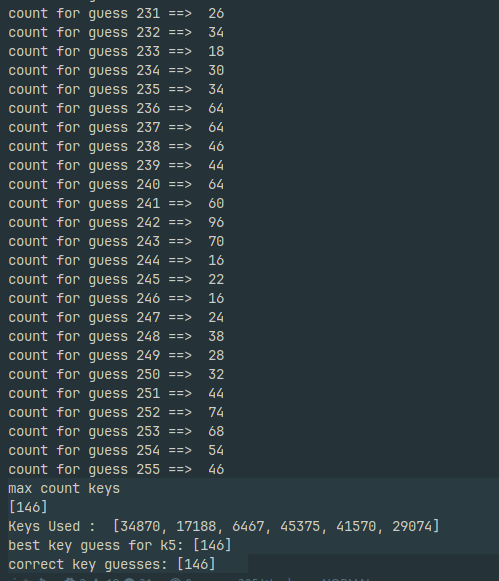
\includegraphics[width=11.2cm]{./p1.png}
    \end{center}

\end{Solution}

%%%%%%%%%%%%%%%%%%%%%%%%%%%%%%%%%%%%%%%%%%%%%%%%%%%%%%%%%%%%%%%%%%
%Complete the assignment now
\end{document}

%%%%%%%%%%%%%%%%%%%%%%%%%%%%%%%%%%%%%%%%%%%%%%%%%%%%%%%%%%%%%%%%%%
%%%%%%%%%%%%%%%%%%%%%%%%%%%%%%%%%%%%%%%%%%%%%%%%%%%%%%%%%%%%%%%%%%